\chapter{Xây dựng UIT-OWL Editor}
\paragraph{Giới thiệu} Qua các chương trước, chúng em đã trình bày các cơ sở lý thuyết từ Semantic Web, Ontology Web Language và giới thiệu khái quát về OWL-API, Vaadin Framework- 2 công cụ chính xây dựng nên ứng dụng chỉnh sửa và phát triển Ontology trên Web mà chúng em tạm gọi là UIT-OWL Editor. Trong chương này, chúng em sẽ trình bày một cách chi tiết nhất có thể về quá trình xây dựng và phát triển nên ứng dụng này.
\section{Bố cục của ứng dụng}
\begin{figure}[h!]
	\centering
	\frame{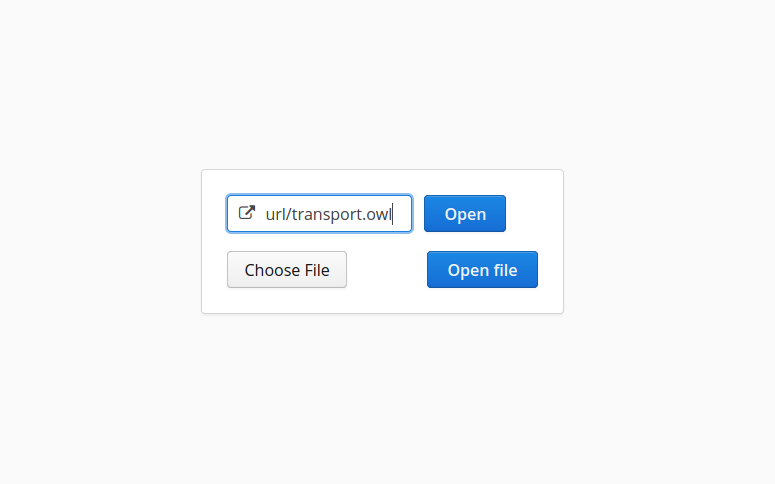
\includegraphics[width=100mm]{Figures/owleditor_entryview.png}}
	\caption{EntryView của UIT-OWL Editor\label{overflow}}
\end{figure}
\begin{figure}[h!]
	\centering
	\frame{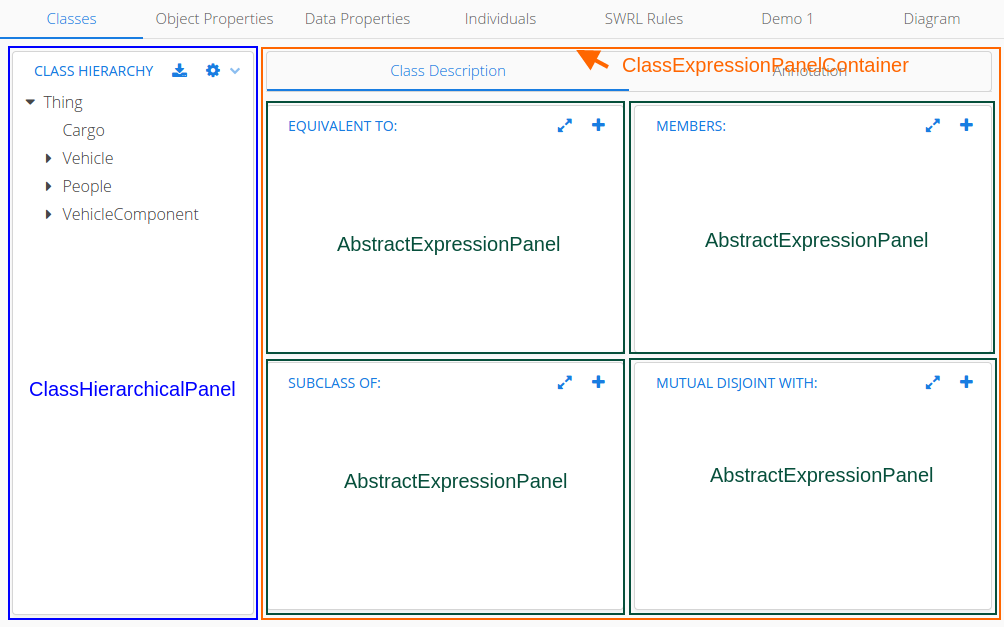
\includegraphics[width=150mm]{Figures/owleditor_mainview.png}}
	\caption{MainView của UIT-OWL Editor\label{overflow}}
\end{figure}
\subsection{OWLEditorUI}
Lớp \textit{OWLEditorUI} thừa kế từ lớp \textit{UI} của Vaadin chính là User Interface của toàn bộ ứng dụng, hoạt động của lớp này tương tự miêu tả của chúng em ở chương trước khi giới thiệu về Vaadin. Chức năng của lớp này gồm:
\begin{enumerate}
	\item Chứa 2 View chính là EntryView và MainView.
	\item Cung cấp đối tượng \textit{OWLEditorKit} cho các UI Component sử dụng qua getter \textit{OWLEditorUI.getEditorKit} nhằm đảm bảo \textit{OWLEditorKit} chỉ khởi tạo 1 lần và chỉ liên kết đến 1 UI là \textit{OWLEditorUI}.
	\item Cung cấp đối tượng \textit{HttpSession} cho các UI Component qua getter \textit{OWLEditorUI.getHttpSession}.
	\item Cung cấp cơ chế reload để nạp ontology mới qua hàm \textit{updateContent}
	\item Cung cấp cơ chế xử lý sự kiện \textit{OWLEditorEventBus} nhằm xử lý các sự kiện cho ứng dụng.
\end{enumerate}
%
\subsection{Các view chính}
Ứng dụng UIT-OWLEditor chỉ gồm 2 View chính:
\begin{description}
\item[Entry View] tương đương với lớp \textit{vn.edu.uit.owleditor.EntryView} trong mã nguồn, là nơi chúng tập nhập vào URL của file OWL2 Ontology hoặc tải file OWL2 Ontology với các định dạng được trình bày trong chương 2. Khi load được ontology \textit{EntryView} sẽ lưu đối tượng \textit{OWLEditorKit} lại trong \textit{HttpSession} phòng trường hợp người dùng mất kết nối với ứng dụn.
\item[Main View] tương đướng với lớp \textit{vn.edu.uit.owleditor.MainView} trong mã nguồn,là giao diện chính của ứng dụng UIT-OWL Editor.
\end{description}
%
\subsection{Các tabsheet trong Main View}
Trong \textbf{MainView} sử dụng Component TabSheet các chứa các Tab tương ứng với các thực thể trong OWL2 Ontology, duy chỉ có 2 Tab cuối dùng để dùng làm demo tính năng phân loại là Tab Demo và Tab cuối cùng là Diagram dùng để vẽ các diagram, đồ thị về phân cấp các đối tượng trong OWL 2 Ontology.

% Class Tab
\subsubsection{Tab Classes} 
\begin{figure}[h!]
	\centering
	\frame{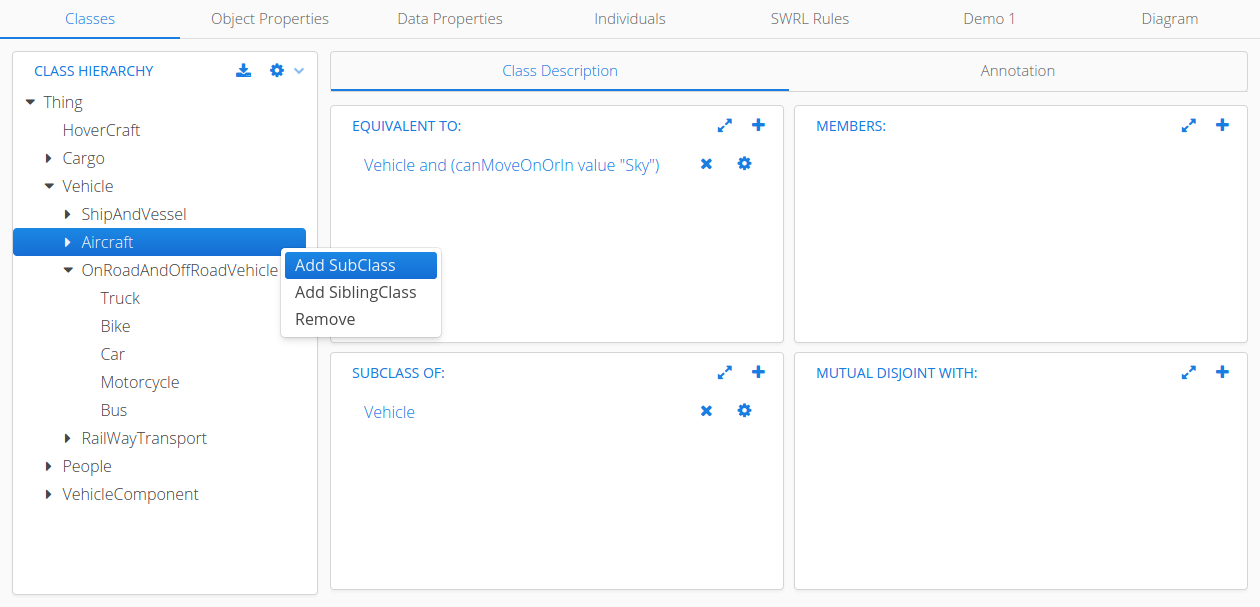
\includegraphics[width=150mm]{Figures/owleditor_classSheet.png}}
	\caption{Class Tab trong UIT-OWL Editor\label{overflow}}
\end{figure}
Tương ứng với lớp \verb|vn.edu.uit.owleditor.view.ClassesSheet| trong mã nguồn. Giao diện sử dụng HorizontalLayout của Vaadin gồm 
\begin{enumerate}
\item Panel bên trái là ClassHierachicalPanel có một cấu trúc dạng cây với các node chính là các lớp nằm trong OWL2 Ontology, với các chức năng thêm/xóa Sub/Sibling Class 
\item Các panel nhỏ bên phải được chứa trong lớp ClassExpressionPanelContainer, mỗ panel thể hiện một mô tả tương ứng với tên của panel đó.
\end{enumerate}	

% Object Property Tab
\subsubsection{Tab Object Properties}  
\begin{figure}[h!]
	\centering
	\frame{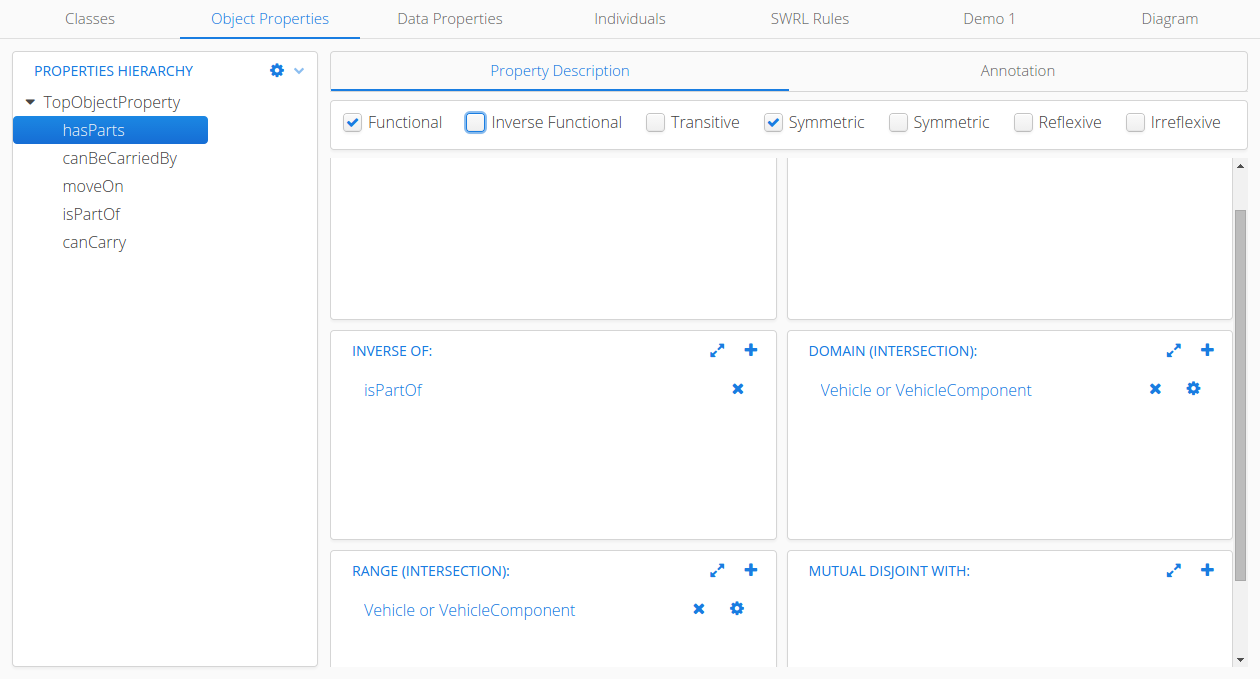
\includegraphics[width=150mm]{Figures/owleditor_opSheet.png}}
	\caption{Object Properties Tab trong UIT-OWL Editor\label{overflow}}
\end{figure}
Tương ứng với lớp \verb|vn.edu.uit.owleditor.view.ObjectPropertiesSheet| trong mã nguồn. Giao diện sử dụng HorizontalLayout của Vaadin gồm 
\begin{enumerate}
\item Panel bên trái là ObjectPropertyHierachicalPanel có một cấu trúc dạng cây với các node đại diện cho các thuộc tính đối tượng trong OWL2 Ontology, với các chức năng thêm/xóa Sibling/Sub Object Property.
\item Một dãy các \textit{CheckBox} dùng để thêm/xóa với các phát biểu trong mục 3.3.6.2 liên quan đến thuộc tính đối tượng được chọn bên trong cấu trúc cây ở bên phải.
\item Các panel nhỏ bên phải được chứa trong lớp ObjectPropertyExpressionPanelContainer, mỗ panel thể hiện một mô tả tương ứng với tên của panel đó về thuộc tính đối tượng đang được chọn trên cấu trúc cây.
\end{enumerate}	

% Data Property Tab
\subsubsection{Tab Data Properties}
\begin{figure}[h!]
	\centering
	\frame{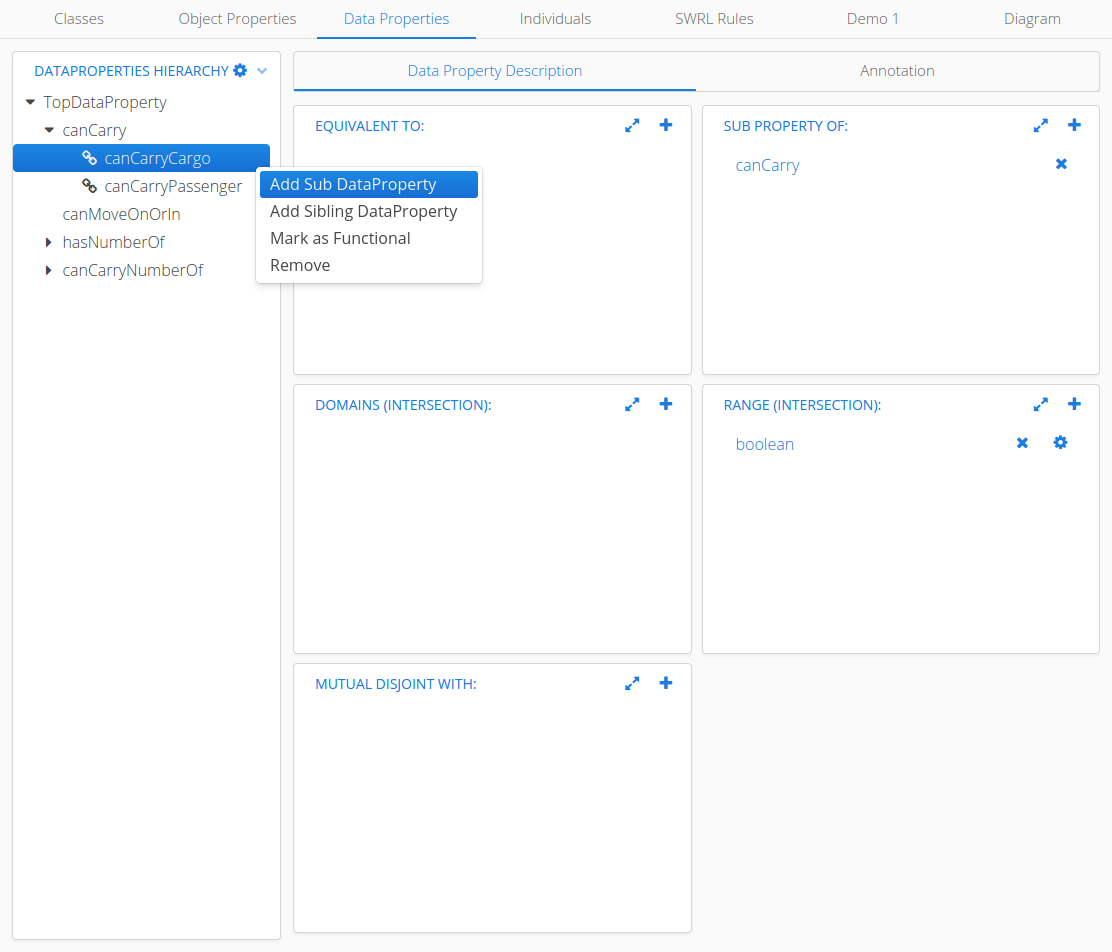
\includegraphics[width=150mm]{Figures/owleditor_dpSheet.png}}
	\caption{Data Properties Tab trong UIT-OWL Editor\label{overflow}}
\end{figure}
Tương ứng với lớp \verb|vn.edu.uit.owleditor.view.DataPropertiesSheet| trong mã nguồn. Các thành phần của tab này gồm:
\begin{enumerate}
\item Panel bên phải là DataPropertyHierachicalPanel có một cấu trúc dạng cây với các node đại diện cho các thuộc tính dữ liệu trong OWL2 Ontology, ngoài chức năng thêm/xóa Sibling/Sub DataProperty còn có tính năng thêm/xóa phát biểu FunctionalDataProperty (những thuộc tính nào có icon phía có nghĩa là có phát biểu FunctionalDataProperty về thuộc tính đó trong ontology.
\item Các panel nhỏ bên phải được chứa trong lớp ObjectPropertyExpressionPanelContainer, mỗ panel thể hiện một mô tả tương ứng với tên của panel đó về thuộc tính dữ liệu đang được chọn bên cấu trúc cây.
\end{enumerate}	

% Individual Tab
\subsubsection{Tab Individual}
\begin{figure}[h!]
	\centering
	\frame{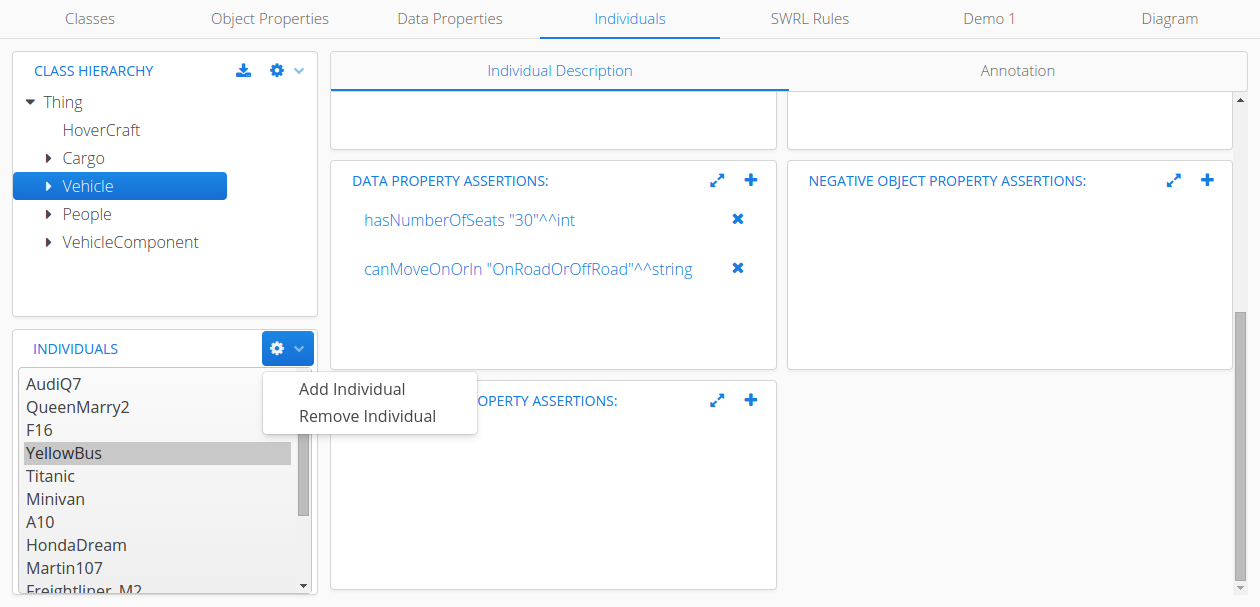
\includegraphics[width=150mm]{Figures/owleditor_individualSheet.png}}
	\caption{Individuals Tab trong UIT-OWL Editor\label{overflow}}
\end{figure}
Tương ứng với lớp \verb|vn.edu.uit.owleditor.view.IndividualsSheet| trong mã nguồn. Các thành phần của tab này gồm:
\begin{enumerate}
	\item Panel bên trái phía trên là ClassHierachicalPanel có một cấu trúc dạng cây với các node chính là các lớp nằm trong OWL2 Ontology, với các chức năng thêm/xóa Sub/Sibling Class. Khi chọn một lớp ở đây thì ListSelect ở bên dưới sẽ hiển thị một danh sách cá thể thuộc lớp này.
	\item Panel bên trái phía dưới là IndividualList hiển thị một danh sách gồm các cá thể thuộc lớp được chọn ở trên, có các tính năng thêm/xóa cá thể.
	\item Các panel bên phải là những panel biểu diễn các phát biểu assertion về cá thể. Tên panel cũng tương ứng với tên phát biểu trong OWL2.
\end{enumerate}

% SWRL Tab
\subsubsection{Tab SWRL}
\begin{figure}[h!]
	\centering
	\frame{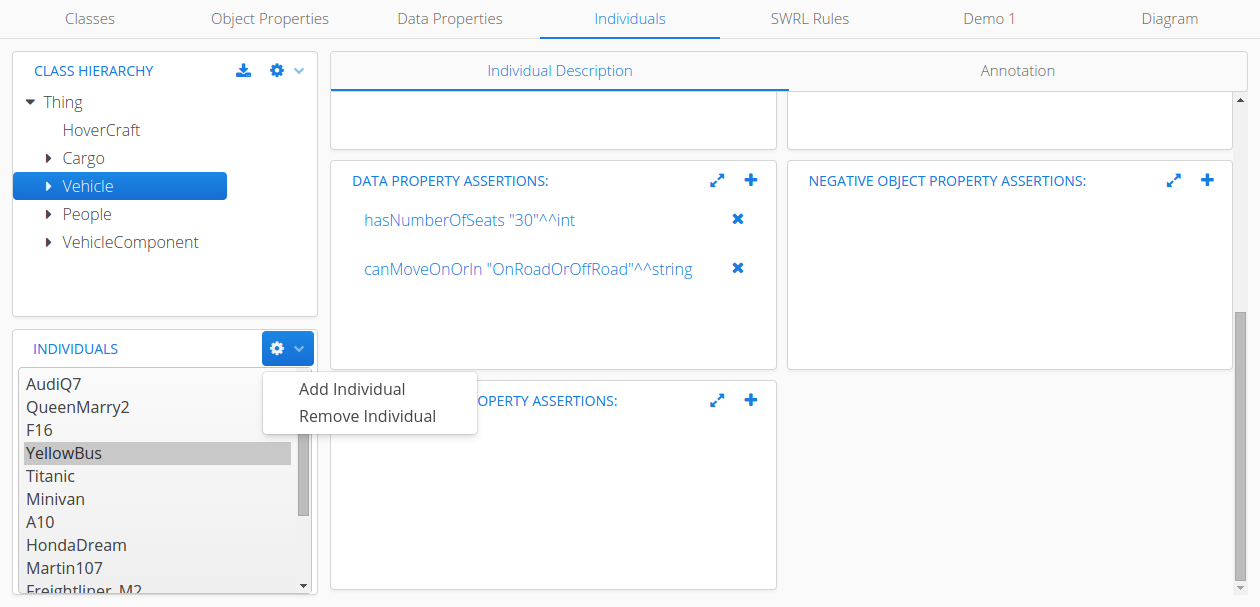
\includegraphics[width=150mm]{Figures/owleditor_individualSheet.png}}
	\caption{SWRL Rule Tab trong UIT-OWL Editor\label{overflow}}
\end{figure}
Tương ứng với lớp \verb|vn.edu.uit.owleditor.view.RuleSheet| trong mã nguồn. Tab này chỉ gồm một thành phần chính là một Table chứa các SWRL trong tài liệu OWL 2 Ontology. Khi right-click sẽ có các chức năng thêm/xóa/sửa rule được chọn.

% Demo Sheet
\subsubsection{Tab Demo}
\begin{figure}[h!]
	\centering
	\frame{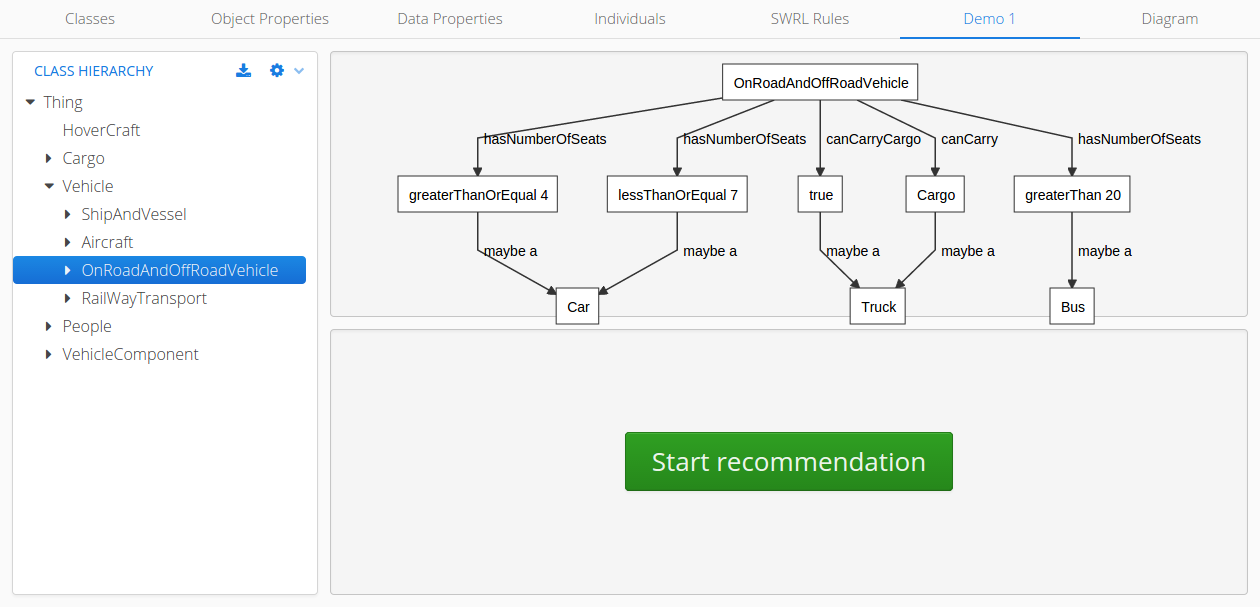
\includegraphics[width=150mm]{Figures/owleditor_demoSheet.png}}
	\caption{Demo Tab trong UIT-OWL Editor\label{overflow}}
\end{figure}
Demo Tab không nằm trong thành phần tiêu chuẩn mà một Ontology Editor bắt buộc phải có như các Tab đã giới thiệu. Tuy nhiên, chúng em cài đặt Demo Tab ở đây với mục đích thử nghiệm tính năng gợi ý phân loại dựa theo SWRL Rule, và sử dụng các Domain và Range restriction để hạn chế các giá trị mà người dùng có thể thêm cho vào cho một cá thể. Các thành phần của tab này gồm:
\begin{enumerate}
\item Panel bên trái là ClassHierachicalPanel.
\item Panel phía trên bên phải sẽ hiện thị một sơ đồ thể hiện gợi ý phân loại cho lớp được chọn.
\end{enumerate}}

\section{OWLEditorKit}
\begin{description}
\item[Interface:] \verb|vn.edu.uit.owleditor.OWLEditorKit|
\item[Class implementation:] \verb|vn.edu.uit.owleditor.OWLEditorKitImpl|
\end{description}
Đây là thành quan trọng nhất của toàn bộ ứng dụng đảm nhiệm việc khai thác các API từ OWL-API, nạp/tạo Ontology từ IRI, suy luận, giải thích các phát biểu, parse các chuỗi viết theo cú pháp \textit{Manchester} thành các mô tả lớp và dữ liệu. Thực ra, các chứng năng vừa kể trên hầu hết đều được thực thi nhờ các API của OWL-API, \textit{OWLEditorKit} đóng gói tất cả lại thành một đối tượng để dễ dàng sử dụng trong các UI Component hơn, cũng như tránh việc phải khởi tạo nhiều lần các API.
\subsection{Các chức năng của OWLEditorKit}

\subsubsection{Load Ontology}
Tương ứng với hàm \textit{loadOntologyFromOntologyDocument}, load các tài liệu OWL2 từ tham số là đối tượng \textit{IRI} của OWL-API, ontology khi load xong sẽ được gán cho đối tượng Active Ontology (sẽ được đề cập ngay sau).
\begin{verbatim}
OWLEditor kit = new OWLEditorKitImpl();
kit.loadOntologyFromOntologyDocument(IRI.create("some url"));
\end{verbatim}
\subsubsection{Giải thích các phát biểu trong OWL2 Ontology}
Tương ứng với hàm \textit{explain}, tham số nhận vào là một phát biểu tương đương đối tượng \textit{OWLAxiom} trong OWL-API. Kết quả trả về là một đối tượng \textit{ExplanationTree} chứa các phát biểu giải thích.

\subsubsection{Xóa các thực thể (Entities) trong OWL2 Ontology}
Xóa các phát biểu trong OWL 2 Ontology không phải là một tác vụ dễ dàng vì một phát biểu có thể được sử dụng để xây dựng nên phát biểu khác. Ví dụ:
\begin{verbatim}
Declaration( Class( A ))
SubClassOf(A B)
EquivalentClasses(A C D)
\end{verbatim}
Giả sử chúng ta muốn xóa phát biểu \textit{Declaration( Class( A ))} thì \textbf{bắt buộc} chúng ta phải xóa luôn những phát biểu có liên quan đến A là \textit{SubClassOf và EquivalentClasses}  bởi vì không có phát biểu khẳng định sự tồn tại của A thì những phát biểu còn lại sẽ trở nên vô nghĩa. Tuy nhiên để thực hiện tác vụ này OWL-API cung cấp cho chúng ta một đối tượng là \textit{OWLEntityRemover} với tính năng duyệt qua mọi phát biểu có liên quan đến thực thể cần xóa, xóa tất cả các phát biểu đó trước khi xóa thực thể. Đối tượng này được sử dụng qua getter \textit{getEntityRemover}.

\subsubsection{Nhà máy sản xuất ra mọi loại đối tượng trong OWL 2 Ontology}
Một chức năng thực sự hữu ích được khai thác từ đối tượng \textit{OWLDataFactory} của OWL-API, với số lượng đối tượng (thực thể, mô tả lớp, thuộc tính, phát biểu, ...) rất lớn để cập ở chương 2, rất khó để chúng ta có thể nhớ và sử dụng chúng dễ dàng. \textit{OWLDataFactory} cung cơ chế để tạo ra mọi loại phát biểu trong OWL 2 Ontology một cách tiện lợi ví dụ như:
\begin{verbatim}
// Declaration( Class(a:Person) )
OWLClass person = factory.getOWLClass("a:Person");

// Declaration( NamedIndividual(a:Peter) )
OWLNamedIndividual Peter = factory.getOWLNameIndividual("a:Peter");

// Declaration( DataProperty(a:HasAge) )
OWLDataProperty hasAge = factory.getOWLDataProperty("a:HasAge");

// ClassAssertion( a:Person a:Peter )
OWLClassAssertionAxiom axiom1 = 
         factory.getOWLClassAssertionAxiom(person, Peter);
         
// "22"^^xsd:integer 
OWLLiteral age = factory.getOWLLiteral(22);

// DataPropertyAssertion( a:HasAge a:Peter "22"^^xsd:integer); 
OWLDataPropertyAssertionAxiom phatbieu = 
         factory.getOWLDataPropertyAssertionAxiom(hasAge, Peter, age);
\end{verbatim}
Trong \textit{OWLEditorKit}, \textit{OWLDataFactory} được truy xuất qua getter \textit{getOWLDataFactory()}.

\subsubsection{Nhà máy sản xuất ra mọi loại đối tượng dữ liệu cho ứng dụng UIT-OWL Editor}
{\let\thefootnote\relax\footnotetext{
		*\textit{http://en.wikipedia.org/wiki/Factory\_method\_pattern}}
}
\begin{description}
\item[Interface:] \verb|vn.edu.uit.owleditor.data.OWLEditorDataFactory|
\item[Class Implementation:] \verb|vn.edu.uit.owleditor.data.OWLEditorDataFactoryImpl|
\end{description}
Học tập mô hình \textit{Factory Pattern} \textsuperscript{*} từ đối tượng \textit{OWLDataFactory}, chúng em cũng tự xây dựng một đối tượng với mục tiêu là cung cấp một cơ chế tiện lợi để tạo ra các đối tượng dữ liệu và các event trong UIT-OWL Editor. Tham số khởi tạo của \textit{OWLEditorDataFactory} chính là \textit{OWLEditorKit}. Ví dụ để tạo sự kiện thêm một phát biểu về lớp vào Ontology:
\begin{verbatim}
// Khởi tạo OWLEditorDataFactory
OWLEditorKit kit = new OWLEditorKit();
OWLEditorDataFactory editorFactory = new OWLEditorDataFactoryImpl(kit);
// Tạo sự kiện thêm phát biểu về lớp
OWLClass person = factory.getOWLClass("a:Person");
OWLClass man = factory.getOWLClass("a:Man");
OWLEditorEvent.ClassAxiomAdded event =
        owlEditorDataFactory.getSubClassOfAddEvent(man, person);
\end{verbatim}
Một cái nhìn chi tiết vào trong \textit{OWLEditorDataFactoryImpl} sẽ làm gì với dòng cuối cùng trong đoạn code ở 
\begin{verbatim}
// Bên trong lớp OWLEditorDataFactoryImpl
private final OWLEditorKit editorKit;
public OWLEditorDataFactoryImpl(OWLEditorKit eKit) {
   this.editorKit = eKit;
}
...
OWLEditorEvent.ClassAxiomAdded getClassAssertionAddEvent(OWLClass owner,
  OWLNamedIndividual expression) {

  return new OWLEditorEvent.ClassAxiomAdded(editorKit.getOWLDataFactory()
                    .getOWLClassAssertionAxiom(owner, expression), owner);
}
\end{verbatim}
Để sử dụng đối tượng \textit{OWLEditorDataFactory}, chúng ta sẽ sử dụng qua getter \textit{OWLEditorDataFactory} của \textit{OWLEditorKit} để tránh khởi tạo nhiều lần (đối tượng này đã được khởi tạo ngay bên trong \textit{OWLEditorKitImpl}.

\subsubsection{Parse chuỗi thành các mô tả lớp (OWLClassExpression)}
OWLEditorKit cũng được tích hợp một đối tượng \textit{ManchesterOWLSyntaxParser} trong OWL-API, nhiệm vụ là để parse các đoạn text từ người dùng theo cú pháp \textit{Manchester} thành các mô tả lớp (OWLClassExpression) hay các miền dữ liệu (OWLDataRange). Parser này được sử dụng thông qua getter \textit{getParser} hoặc parse trực tiếp qua hàm \textit{parseClassExpression(String stringToParse)} . Ví dụ:
\begin{verbatim}
OWLEditorKit eKit = new OWLEditorKitImpl();
// nạp ontology ...
// Cách 1
ManchesterOWLSyntaxParser parser = eKit.getParser();
parser.setStringToParse("Has some Friend");
OWLClassExpression ce1 = parser.parseClassExpression();
// Cách 2 
OWLClassExpression ce2 = eKit.parseClassExpression("Has some Kid");
\end{verbatim}

\subsubsection{Suy luận các phát biểu}
Tính năng suy luận được đáp ứng bới Pellet Reasoner đề cập ở chương trước. Reasoner cũng đã được tạo sẵn trong \textit{OWLEditorKitImpl}, truy cập thông qua getter \textit{getReasoner()} và sử dụng như mô tả ở chương trước.

\subsubsection{Áp dụng các thay đổi về phát biểu cho ontology}
Chức năng này được thực thi bởi đối tượng \textit{OWLOntologyManager} được khởi tạo cùng với lớp \textit{OWLEditorKitImpl}, sử dụng thông qua getter \textit{getModelManager()}.
\textit{OWLOntologyManager} sẽ được sử dụng để áp dụng thay đổi trong các hàm Subscriber (sẽ được đề cập trong phần Xử lý sự kiện).

\subsection{Một số đối tượng đáng chú ý khác trong OWLEditorKitImpl}
Ngoài các chức năng đi kèm với các đối tượng quan trong kể trên trong implementation của \textit{OWLEditorKit} cũng có một số đối tượng mà chúng ta cũng cần phải lưu ý.
\subsubsection{Active Ontology}
Biến  \textit{activeOntology} là một đối tượng \textit{OWLOntology} của OWL-API được khai báo trong \textit{OWLEditorKitImpl}. Biến này chính là OWL2 Ontology hiện hành đang được thao tác trên giao diện. Các thao tác thêm/xóa/sửa các phát biểu qua các giao diện đều sẽ được cập nhật và áp dụng lên đối tượng \textit{OWLOntology} này.
\subsubsection{Manchester Renderer}
Hàm static \textit{OWLEditorKitImpl.render(OWLObject)} dùng render hay chuyển đổi các đối tượng OWL 2 thành dạng chuỗi (cú pháp Manchester), chủ yếu để render các phát biểu, mô tả lớp/thuộc tính/kiểu dữ liệu.
\subsubsection{Lấy tên thực thể}
Hàm static \textit{OWLEditorKitImpl.getShortForm(OWLEntity)} dùng lấy tên các đối tượng \textit{OWLEntity}. Ví dụ: \textit{longIRI:Person} -> \textit{Person}


\section{Xử lý sự kiện trong UIT-OWL Editor}
Qua phần đầu tiên về bố cục của ứng dụng, cũng có thể thấy với nhiều Tab và các Panel như vậy thì việc xây dựng các Event (sự kiện) và các EventListener sẽ đòi hỏi một công sức khá lớn nếu viết theo kiểu truyền thống Java. Vì thế chúng em đã chọn một cách tiếp cận khác đó sử dụng thư viện Google Guava EventBus \cite{guava}. Thư viện này cho phép nhanh chóng đăng ký (register) một hàm subscriber trong một UI Component để biến nó thành EventListener, sự kiện có thể đến từ bất kì component nào khác mà chúng ta không nhất thiết phải quan tâm vì đã có \textit{OWLEditorEventBus} xử lý. Cái chúng ta cần quan tâm đó là kiểu của đối tượng event được post (truyền lên) EventBus. Trong ứng dụng của chúng em, việc sử dụng  \textit{Guava EventBus} được đơn giản hóa bằng các hàm tĩnh nằm trong \textit{OWLEditorEventBus}.
Dòng sự kiện trong hầu hết các UI Component của ứng dụng sẽ giống như hình sau:
\begin{figure}[h!]
	\centering
	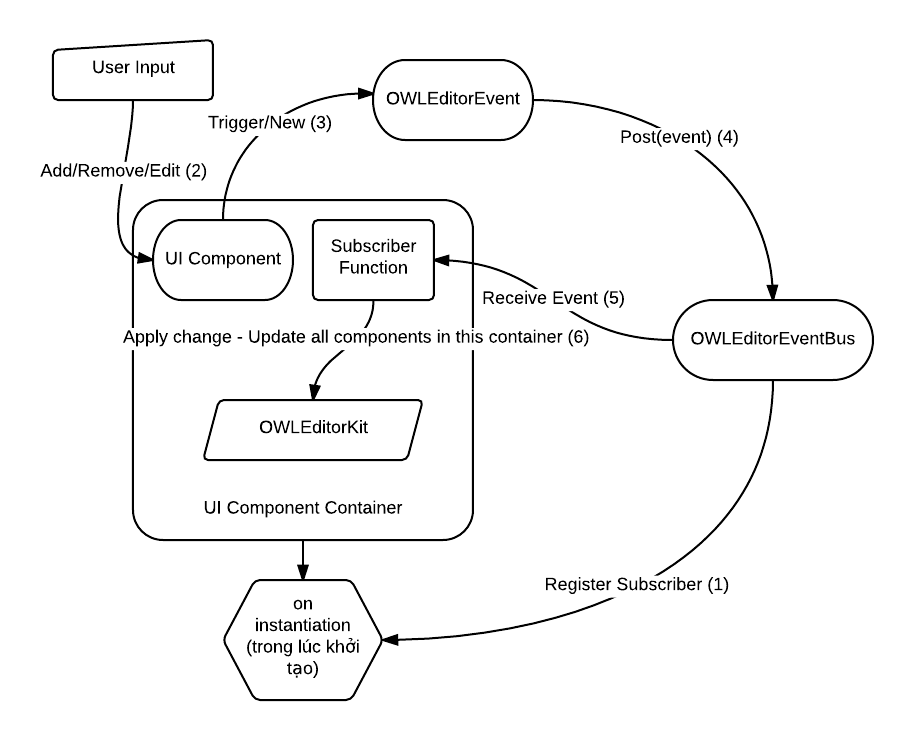
\includegraphics[width=120mm]{Figures/eventBusChart.png}
	\caption{Dòng sự kiện trong UIT-OWL Editor\label{overflow}}
\end{figure}
Chúng em xin lấy một \textit{ClassExpressionPanelsContainer} ra làm ví dụ:


























